\chapter{Definition and Literature Review}
\label{Chapter2}

% 转折
% \subsubsection{Approximate Bayesian Inference Intuition}
\section{Bayesian Inference Paradigm}
\label{bayeisanP}
\textbf{Why Bayesian}
Bayesian Inference approaches shares numerous advantages in statistic community and applicationa areas, particularly for the circumstance when there is lack of data. An appropriate prior choice can be beneficial in aforementioned case, especially for medical problem where the amount of effective data is extremely rare and untenable. Additionally, unlike frequentist inference approaches which treat parameter estimate as a fixed value, Bayesian Inference approaches regard parameter estimate as a random variable that have probability distribution, which means interval estimate and error variance would be generated for capturing uncertainty, offering  belief and confidence for interpretating parameter estimates.

\textbf{Bayesian Inference Intuition}
Bayesian inference approach stems from the Bayes rule, which is defined as Equation (\ref{eq:Bayesrule}) based on theory developed by \cite{Beech1959}. Suppose $\theta$ is our model parameter of interest, $\mathcal{D}$ is data, then $p(\theta)$ is known as prior distribution, which offers pre-existing knowledge or information about $\theta$. Posterior distribution $p(\theta|\mathcal{D})$ refers to the likelihood conditioning on the data $\mathcal{D}$.
Incorporating information from current data and prior knowledge, posterior distribution can be then inferred and simplified to Equation (\ref{eq:simBayesrule}) since $p(\mathcal{D})$ is equal to constant and is also insignificant to know overall posterior distribution.
\begin{equation}
	p(\theta|\mathcal{D}) \propto p(\mathcal{D}|\theta)p(\theta),
	\label{eq:simBayesrule}
\end{equation}




\section{Least Absolute Shrinkage and Selection Operator(LASSO) penalized regression}
\subsection{Lasso penalty formulation}
The constraint form of lasso can be shown by Equation \ref{eq:lasso2}, where $t \geq 0$ is denoted as a tuning term $t$, regression coefficient is $\beta$, $||\beta||_1$ is the $l_1$ norm of beta, $||\beta||_2$ is the $l_2$ norm of $\beta$, data matrix is $X$, response variable is $y$. The estimation for lasso estimate $\hat{\beta}_{lasso}$ is defined by Equation \ref{eq:lasso2}. 

\begin{equation}
	\label{eq:lasso2}
	\hat{\beta}_{lasso} = \underset{\beta}{\operatorname{argmin}} ||y-X\beta||_2, s.t. ||\beta||_1 \leq t, t \geq 0.
\end{equation}
In order to transform constraint form of lasso to penalty form, Lagranage multiplier method, as a pivotal technique from transforming a constraint optimization system into an unconstrained penalty formulation of system has been used. The Lagrangian function for constrained Lasso Regression is constructed by Equation \ref{eq:lagrangelasso}
\begin{equation}
	\label{eq:lagrangelasso}
	\mathcal{L}(\beta,\lambda) =  ||y-X\beta||_2 + \lambda||\beta||_1 - \lambda t, \lambda \geq 0
\end{equation}
Since the objective function contains a quadratic term $||y-X\beta||_2$ with a linear term $\lambda||\beta||_1 - \lambda t)$, leading to a convex optimization problem. Due to strong duality theorem in convex optimization system, therefore the penalty formulation of lasso regression can be deduced as Equation \ref{eq:lasso1}, is equivalent to constraint form \ref{eq:lasso2} after ignoring the unaffected constant $-\lambda t$.


Graphical demonstration of the lasso for Equation \ref{eq:lasso2} and Equation \ref{eq:lasso1} can also be found on the left hand side of the Figure \ref{fig:lassodemo}, where the squared constraint set is drawn, in addition to the contour line of regression coefficient. Given that $\lambda$ is set as penalty term that control the strength of penalization, larger penalization facilitate a more sparse solution, so that further enclosing the estimated coefficient to lies on the axis of each parameter as shown in Figure \ref{fig:lassodemo}. Lasso regression coefficient would have higher chance to render the contour line of $\beta$ intersect with the corner of the squared constraint set, causing the occurrence of sparse estimated regression coefficient. Compared with the ridge regression where a sum of square of penalty term is yielded instead on the right side of Figure \ref{fig:lassodemo}, ridge regression tends to gain a non-sparse solution due to circled constraint set for $\beta$.

\begin{figure}
	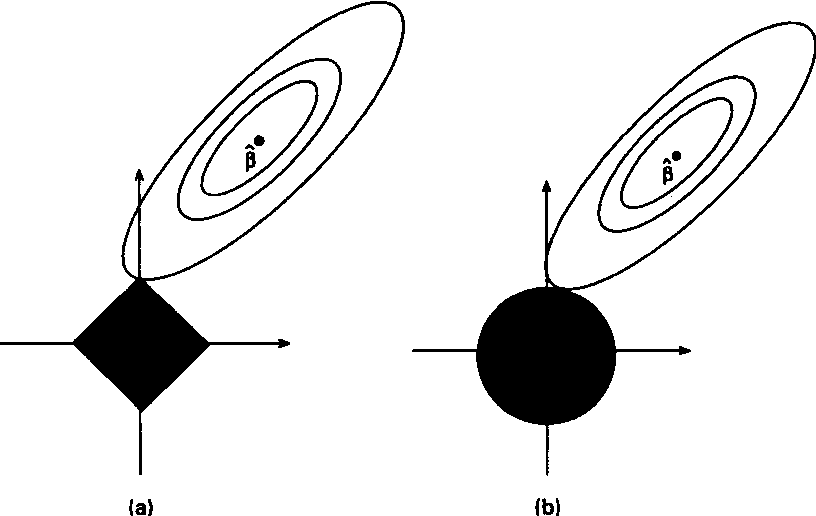
\includegraphics[width=\linewidth]{lassodemo}
	\caption{Graphical comparison between lasso regression and ridge regression}
	\label{fig:lassodemo}
\end{figure}

\textbf{Problem}
In addition, the optimal estimated $\beta_{lasso}$ can be generated by taking the derivative with respect to $\beta$ and solving the normal equation, denoted as Equation (\ref{eq:lassosolution}).
In addition, lasso estimated can be efficiently computed via Least Angle Regression algorithm by


\section{Bayesian Lasso}
\subsection{Bayesian Lasso model}
\cite{park_casella_2008} has proposed an alternative conditional Laplace prior formula of the form Equation (\ref{eq:LassoPrior}), expanded by Equation(\ref{eq:expandLasso})
\begin{equation}
	\label{eq:expandLasso}
	\pi(\beta) = \prod_{j=1}^p \frac{\lambda}{2} e^{-\lambda|\beta_j|}
\end{equation}

For a given variance, the mode of  posterior form in Equation(\ref{eq:fullCondLasso}) is consistent with the estimate of lasso equation in \ref{eq:lasso1}, but it will hinder the bayesian interpretation, inference and variable selection since the bayesian predictive distribution make future inference via a posterior mean instead of posterior mode.
In addition, if a variance is unknown, the posterior will be a multimodal distribution, the derivation has been provided by the appendeix from \cite{park_casella_2008}.
\begin{equation}
	\label{eq:fullCondLasso}
	\pi(\beta,\sigma^2|\tilde{y}) \propto \pi(\sigma^2)(\sigma^2)^{-(n-1)/2}\textnormal{exp}(\frac{1}{2\sigma^2}(\tilde{y}-X\beta)^T(\tilde{y}-X\beta)-\lambda\sum_{j=1}^p|\beta_j|)
\end{equation}
\begin{equation}
	\label{eq:lassocondprior}
	\pi(\beta |\sigma^2) = \prod_{j=1}^p \frac{\lambda}{2\sqrt{\sigma^2}} e^{-\lambda|\beta_j|/\sqrt{\sigma^2}}
\end{equation}
To remedy this issue, a conditional Laplacian prior from \ref{eq:lassocondprior} with respect to Equation(\ref{eq:expandLasso}) has been designed, ensuring the unimodality of the posterior for $\beta$, and the current prior with respect to $\beta$, $\sigma^2$  can be written in 
\begin{equation}
	\label{eq:lassoprior}
	\pi(\beta,\sigma^2) \propto \pi(\sigma^2) \prod_{j=1}^p \frac{\lambda}{2\sqrt{\sigma^2}} e^{-\lambda|\beta_j|/\sqrt{\sigma^2}}
\end{equation}
which can result in the unimodal joint posterior distribution $\pi(\beta,\sigma^2|\tilde{y})$ of $\beta$ and $\sigma^2 > 0$ under the new prior \ref{eq:lassoprior}, given an improper prior selection for $\pi(\sigma^2) = \frac{1}{\sigma^2}$ and $\lambda \geq 0$
Additionally, an additional latent variable $\tau$ are introduced as a scale mixture of Gaussians for reformulation of conditional prior \ref{eq:lassocondprior} as \ref{eq:MofN}, which can be regarded as corresponding weight assigned to each regression coefficient. If $\tau_j$ goes to 0 then the corresponding regression coefficient will be shrunk towards zero accordingly.
\begin{equation}
	\label{eq:MofN}
	\frac{\alpha}{2}e^{-\alpha|z|} = \int_{0}^{\infty} \frac{1}{\sqrt{2\pi s}}e^{-z^2/(2s)} \frac{\alpha^2}{2}e^{-\alpha^2s/2}ds, \alpha > 0
\end{equation}

Finally, the hierarchical bayesian lasso model functional form can be written as Equation (\ref{eq:blassocond}).
\begin{equation}
	\label{eq:blassocond}
	\begin{multlined}
	y|\mu,X,\beta,\sigma^2 \sim N_n(\mu + X\beta,\sigma^2I)\\
	\beta|\tau_1^2,...,\tau_p^2 \sim N_p(0,\sigma^2D_{\tau})\\
	D_{\tau} = diag(\tau_1^2,...,\tau_p^2)\\
	\tau_1^2..,\tau_p^2 \sim \prod_{j=1}^p \frac{\lambda^2}{2} e^{-\lambda^2\tau_j^2/2}d\tau_j^2, \tau_1^2,..,\tau_j^2 > 0\\
	\sigma^2 \sim \pi(\sigma^2) = 1/\sigma^2, \sigma^2 > 0\\.
	\end{multlined}
\end{equation}

\subsection{Bayesian Lasso Gibbs Sampler}
\subsubsection{Gibbs Sampler}
Gibbs sampler is a Markov Chain Monte Carlos sampling algorithm for efficient sampling of any probability density function, given corresponing conditioal distribution form with an reasonable burn-in period. For each iteration, each parameter of interest will be sampled once by conditional distribution for the current iteration. After reasonable burn-in period, it will return an exact posterior distribution after discarding samples generated before burn-in period.
After completion, the combination of each component of samples can formulate full samples of posterior distribution. As a result, the functional form of conditional distribution given any other parameter of interest has to be acquired. For the bayesian lasso model, this means the following exact functional form has to be derived
\begin{equation}
	\begin{multlined}
	p(\mathbf{\beta}|\mathcal{D},\sigma^2,\mathbf{\tau})\\
	p(\mathbf{\sigma}|\mathcal{D},\sigma^2,\mathbf{\tau})\\
	p(\mathbf{\tau_j}|\mathcal{D},\sigma^2,\mathbf{\tau})\\
	\end{multlined}
\end{equation}
After getting functional form and ignoring the normalizing constant, we can infer their category of probability distribution for each expression, and we can sample from the corresponding distribution.

\textbf{Initial Setting}:
Before derivation, we would like to formulate our initial setting: $\lambda$ is fixed, $\pi(\sigma^2) = \frac{b^a}{\Gamma(a)} (\sigma^2)^{-a-1}e^{-b^2/\sigma^2},\sigma^2>0,a>0,b>0$ follows an Gamma distribution with parameter $a$ and $b$. \\
Our first step is to write full posterior distribution: $p(\mathbf{\beta},\mathbf{\tau},\sigma^{2},\mathcal{D})$

\textbf{Joint distributional form}:
Given Equation \ref{eq:blassocond}, we can write joint distribution form as
\begin{equation}
	\begin{multlined}
		p(\tilde{y},\beta,\tau,\sigma^2) = p(\tilde{y}|\beta,\sigma^2,\tau)p(\sigma^2)\prod_{j=1}^p p(\beta|\sigma^2,\tau_j)p(\tau_j^2)\\
		=\frac{1}{(2\pi\sigma^2)^{\frac{n}{2}}} e^{\frac{-(\tilde{y} -X\beta)^T(\tilde{y}-X\beta)}{2\sigma^2}}
		\frac{b^a}{\Gamma(a)} (\sigma^2)^{-a-1}e^{-b^2/\sigma^2}
		\prod_{j=1}^p \frac{1}{(2\sigma^2\tau_j^2)^{1/2}}e^{-\frac{-1}{2\sigma^2\tau_j^2}\beta_j^2}\frac{\lambda^2}{2}e^{-\lambda^2\tau_j^2/2}
	\end{multlined}
\end{equation}

\textbf{Formulation of $\beta$}:

\begin{equation}
	\begin{multlined}
		p(\beta | \tilde{y},\tau,\sigma^2) \propto  	p(\tilde{y},\beta,\tau,\sigma^2)
	\end{multlined}
\end{equation}
Recognizing the term without $\beta$ as constant, the conditional distribution of $\beta$ can be simplified to
\begin{equation}
	\begin{multlined}
	p(\beta|\tilde{y},\sigma^2,\tau) \propto \textnormal{exp}(\frac{\beta^TX^TX\beta - 2y^TX\beta +\lambda^2\beta^TA^{-1}\beta}{-2\sigma^2}), A = diag(\tau)\\
	=  \textnormal{exp}(-\frac{1}{2}\beta^T(\frac{X^TX + \lambda^2A^{-1}}{-2\sigma^2})\beta + \frac{\tilde{y}^TX\beta}{\sigma^2})\\
	\sim \textnormal{MVN}(\mu^*,\Sigma^*)\\
	\textnormal{where } \mu^* = (X^TX+\lambda^2A^{-1})^{-1}X^Ty, \Sigma^* = (X^TX+\lambda^2A^{-1})^{-1}\sigma^2\\
	\end{multlined}
\end{equation}
So we can sample $\beta$ from a multivariate normal distribution with its corresponding mean and variance.

\textbf{Formulation of $\sigma^2$}:

\begin{equation}
	\begin{multlined}
		p(\sigma^2|\tilde{y},\beta,\tau) \propto  	p(\tilde{y},\beta,\tau,\sigma^2)  \\
		= (\sigma^2)^{-\frac{n}{2}-\frac{p}{2}-a-1}\textnormal{exp}(-\frac{1}{2\sigma^2}(\tilde{y}-X\beta)^T(\tilde{y}-X\beta)+\frac{1}{2\sigma^2}\beta^TD_{\tau}\beta+\frac{b}{\sigma^2}).\\
		\sim \textnormal{Inverse-Gamma}(\alpha^*,\beta^*)\\
		\textnormal{where } \alpha^* = \frac{n}{2}+\frac{p}{2}+a, \beta^* = 
		(\tilde{y}-X\beta)^T(\tilde{y}-X\beta)/2 + \beta^TD_{\tau}\beta/2 +b
	\end{multlined}
\end{equation}

\textbf{Formulation of $\tau_j$}:

\begin{equation}
	\begin{multlined}
		p(\tau_j|\tilde{y},\beta,\sigma^2) \propto  	p(\tilde{y},\beta,\tau,\sigma^2)  \\
		= \frac{1}{\sqrt{\frac{2\pi\sigma^2\tau_j}{\lambda^2}}}\textnormal{exp}(-\frac{-\beta_j^2\lambda^2}{2\sigma^2\tau_j})\textnormal{exp}(-\frac{1}{2}\tau_j)]
		\sim GIG(a^*,b^*,p^*)\\
		\textnormal{where GIG is generalized inverse gaussian distribution } a^* = 1, b^* = \frac{\beta_j^2\lambda^2}{\sigma^2}, p = \frac{1}{2}
	\end{multlined}
\end{equation}

\textbf{Summary}
In summary, each conditional distribution can be written in the following equation
\begin{equation}
	\label{eq:lassoposteriorsummary}
	\begin{multlined}
		p(\beta |y,\sigma^2,a): \textnormal{MVN}((X^TX+\lambda^2A^{-1})^{-1}X^Ty,(X^TX+\lambda^2A^{-1})^{-1}\sigma^2)\\
		p(\sigma^2 |y,\beta,\tau_j):\textnormal{Inverse-Gamma}(\frac{n}{2}+\frac{p}{2}+a,\frac{||y-X\beta||_2^2}{2}+\frac{\lambda^2\sum_j{\beta_j^2}}{2\tau_j}+b)\\	
		p(\tau_j|y,\beta,\sigma^2): GIG(1,\frac{\beta_j^2\lambda^2}{\sigma^2},1/2)\\
	\end{multlined}
\end{equation}
The gibbs sampler can be established by the following algorithm.
\begin{algorithm}
	\caption{Gibbs Sampler for the Bayesian Lasso}
	\begin{algorithmic}[1]
		
		\State Given $\lambda^2>0, \mathbf{\tau}^{(1)} = \mathbf{1_n}, \sigma^{2(1)} =1 , t=1$ \Comment{Initial Setting}
		\While{$t \leq 10^5$}
		
		\State Sampling $\mathbf{\beta}^{(t+1)} \sim \textnormal{MVN}((X^TX+\lambda^2A^{-1})^{-1}X^Ty,(X^TX+\lambda^2A^{-1})^{-1}\sigma^2) $  \Comment{Generate sample $\beta$}
		\State Sampling $\sigma^{2(t+1)} \sim IG(\frac{n}{2}+\frac{p}{2}+a,\frac{||y-X\beta||_2^2}{2}+\frac{\lambda^2\sum_j{\beta_j^2}}{2\tau_j}+b)$ \Comment{Generate sample $\sigma^2$}
		\For{$j$=1,...,$p$}
		\State Sampling $\mathbf{\tau}_j^{(t+1)} \sim GIG(1,\frac{\beta_j^2\lambda^2}{\sigma^2},1/2)$ \Comment{Generate sample $\tau_j$}
		\EndFor
		\State $t \leftarrow t + 1$
		\EndWhile  \label{roy's loop}
		
		
	\end{algorithmic}
\end{algorithm}

% \section{Bayesian Paradigm}
\textbf{Automatic selection of the penalty parameter $\lambda$}
Common choice of penalty parameter $\lambda$ in the non-bayesian paradigm involves cross-validation approach, which is time-consuming and computational challenging especially for large datasets.
\cite{park_casella_2008} arrange a hyperprior to $\lambda^2$ from Gamma distribution as \ref{eq:hyperprior}. 
According to \cite{park_casella_2008}, there are some additional notification of choosing prior, which involves: firstly, to avoid mixing issue, the prior distribution for $\lambda^2$ should reach zero asymptotically with a descent speed as $\lambda^2 $ goes to infinity, Secondly, the density at maximum likelihood estimate should be assigned with enough probability density with a overall flat distribution.
\begin{equation}
	\label{eq:hyperprior}
	\pi(\sigma^2) = \frac{\delta^\gamma}{\Gamma(\gamma)}(\lambda^2)^{\gamma-1}e^{-\delta\lambda^2}, \textnormal{for } \delta>0, \gamma>0, \lambda^2>0
\end{equation}

 The penalty parameter is the extent of penalization of non-zero coefficient, which is also a compromise between model simplicity and fitting capability to data in the frequentist lasso setting. According to the posterior form of $\tau_j$, $\lambda$ controls the shape of generalized inverse-Gaussian posterior distribution of $\tau_j$ as shown in the \ref{eq:lassoposteriorsummary}.

To obtain the posterior form of $\lambda$, we need to incorpoate a proper hyperprior distribution to the joint distribution $p(y,\beta,\sigma^2,\tau)$ first, assuming the gamma distribution has shape $\theta$ and rate parameter $\gamma$.
\begin{equation}
\end{equation}
\begin{equation}
	\label{eq:hyperpriorGamma}
	\begin{multlined}
	p(\lambda|\tilde{y},\beta,\sigma^2,\tau) \propto  	p(\tilde{y},\beta,\tau,\sigma^2,\lambda)  \\
	= (\prod_{j=1}^p \frac{\lambda^2}{2} e^{-\lambda^2\tau_j^2/2})(\lambda^2)^{\gamma-1}e^{-\delta\lambda^2}\\
	= (\lambda^2)^{p+\gamma-1}e^{-\lambda^2(\frac{1}{2}\sum_{j=1}^p \tau_j^2+\delta)}
\end{multlined}
\end{equation} 
Thus, the posterior distribution of $\lambda$ is still following a Gamma distribution, with a shape parameter $p+\gamma-1$ and rate parameter $\sum_{j=1}^p \tau_j^2+\delta)$. The $\lambda^2$ can be sampled by \ref{eq:hyperpriorGamma}, based on using an Augmented Gibbs sampler.

\section{Expectation Maximization}
\subsection{Bayesian Expectation Maximization}


\section{Variational Inference}
\label{VI}

\subsection{Mean Field Variational Bayes(MFVB)}
Suppose there are $n$ number of parameters, then MFVB assumes target distribution $q(\theta)$ is the product of single factorization of each parameter distribution $q_i(\theta_i)$, due to simplicity of product density form. 
\begin{equation}
	q(\theta) = \prod_{i=1}^{n} q_i(\theta_i)
\end{equation}
To measure the similarity between true distribution and target distribution, KL divergence metric is selected to produce

\begin{equation}
	KL(q(x)||p(x|\mathcal{D})) 
\end{equation}

\subsection{MFVB for Bayesian Lasso}







